\section{Vibrations And Noise}
Vibrations are of great concern in the development of quadrotor flight controllers, and even more so when introducing variable pitch. The addition of variable pitch mechanisms increases the mechanical complexity of the quadrotor by adding more moving parts, thus creating more sources of vibrations.
\\
\\
On a quadrotor, the four individual motors generate vibrations which are carried through the frame and affects stabilization by disturbing the readings of the inertial measuring unit. If vibrations become to severe, stabilization will be difficult to achieve.
\\
\\
Bench testing shows that the vibrations increase significantly when the variable pitch mechanisms are attached to the motors. It is therefore important that all other sources of vibrations are minimized as much as possible. The frame, holes, parts and mechanical linkages therefore have to be as made as precise as possible. 
\\
\\
The commercial variable pitch mechanisms used in this project does also show imperfections. On high RPM, the inner shafts vibrates uncontrollably resulting in major disturbances in the IMU.
\\ 
\\
In order to minimize the vibration issues, counter measures must be taken. There are several ways of reducing vibrations and noise, mechanical, electrical and software counter measures must be taken.


\subsection{Mechanical Counter Measures}
The bench testing shows that if the vibrations in the frame are severe enough the propeller gets vibrations and the trust is affected. This was the case when the variable pitch mechanism got attached. The thrust had to be limited to 50\% in order to limit the vibration in the propeller. The vibration seem to stem from jerky parts in the mechanism itself. This is the biggest limitation of the agility to the quadrotor.
 \\
 \\
Figure \ref{fig:yo} shows how severe the raw yaw gyro data is when the quad is flat on a table, and the thrust is slowly increased to the maximum.
\begin{figure}[H]
    \centering
         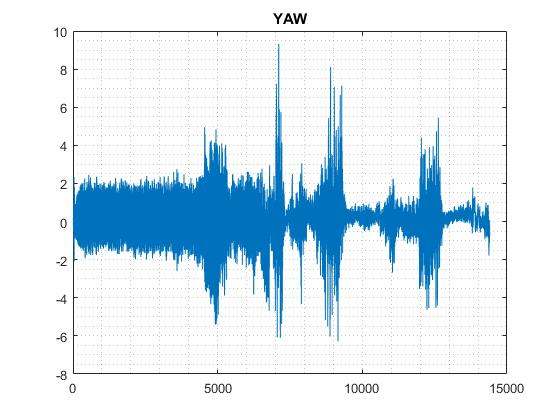
\includegraphics[width = 0.6\textwidth]{NoisePictures/YAWshaftTrow.jpg}
      \caption{Gyroscope yaw raw data}
    \label{fig:yo}
\end{figure} 
These vibrations is probably due to to low precision in the variable pitch mechanism itself. The variable pitch mechanism introduces enormous vibrations. Having access to machinery that can develop the VP mechanism with the highest possible precision is probably a requirement if variable pitch control of quadrotors should be worth the additional mechanical complexity and work properly. Commercial available variable pitch mechanical seems to be made of way to low precision.
\\
\\
The mounting of the is IMU very important, it must be mounted in the center of the quadrotor because the vibrations will be least in that place. The IMU also has to be mounted on a material, which absorbs the worst vibrations. i.e foam or double sided tape.
\\
\\
Figure \ref{fig:PIKK2} shows the mounting of the IMU. The IMU is mounted with a tripple material dampening setup. Both the IMU and the prototype board is mounted with double sided tape which absorbs vibrations. The sandwich is mounted on a Rubber damper. The setup is seen in figure \ref{fig:PIKK2}.
\begin{figure}[H]
    \centering
         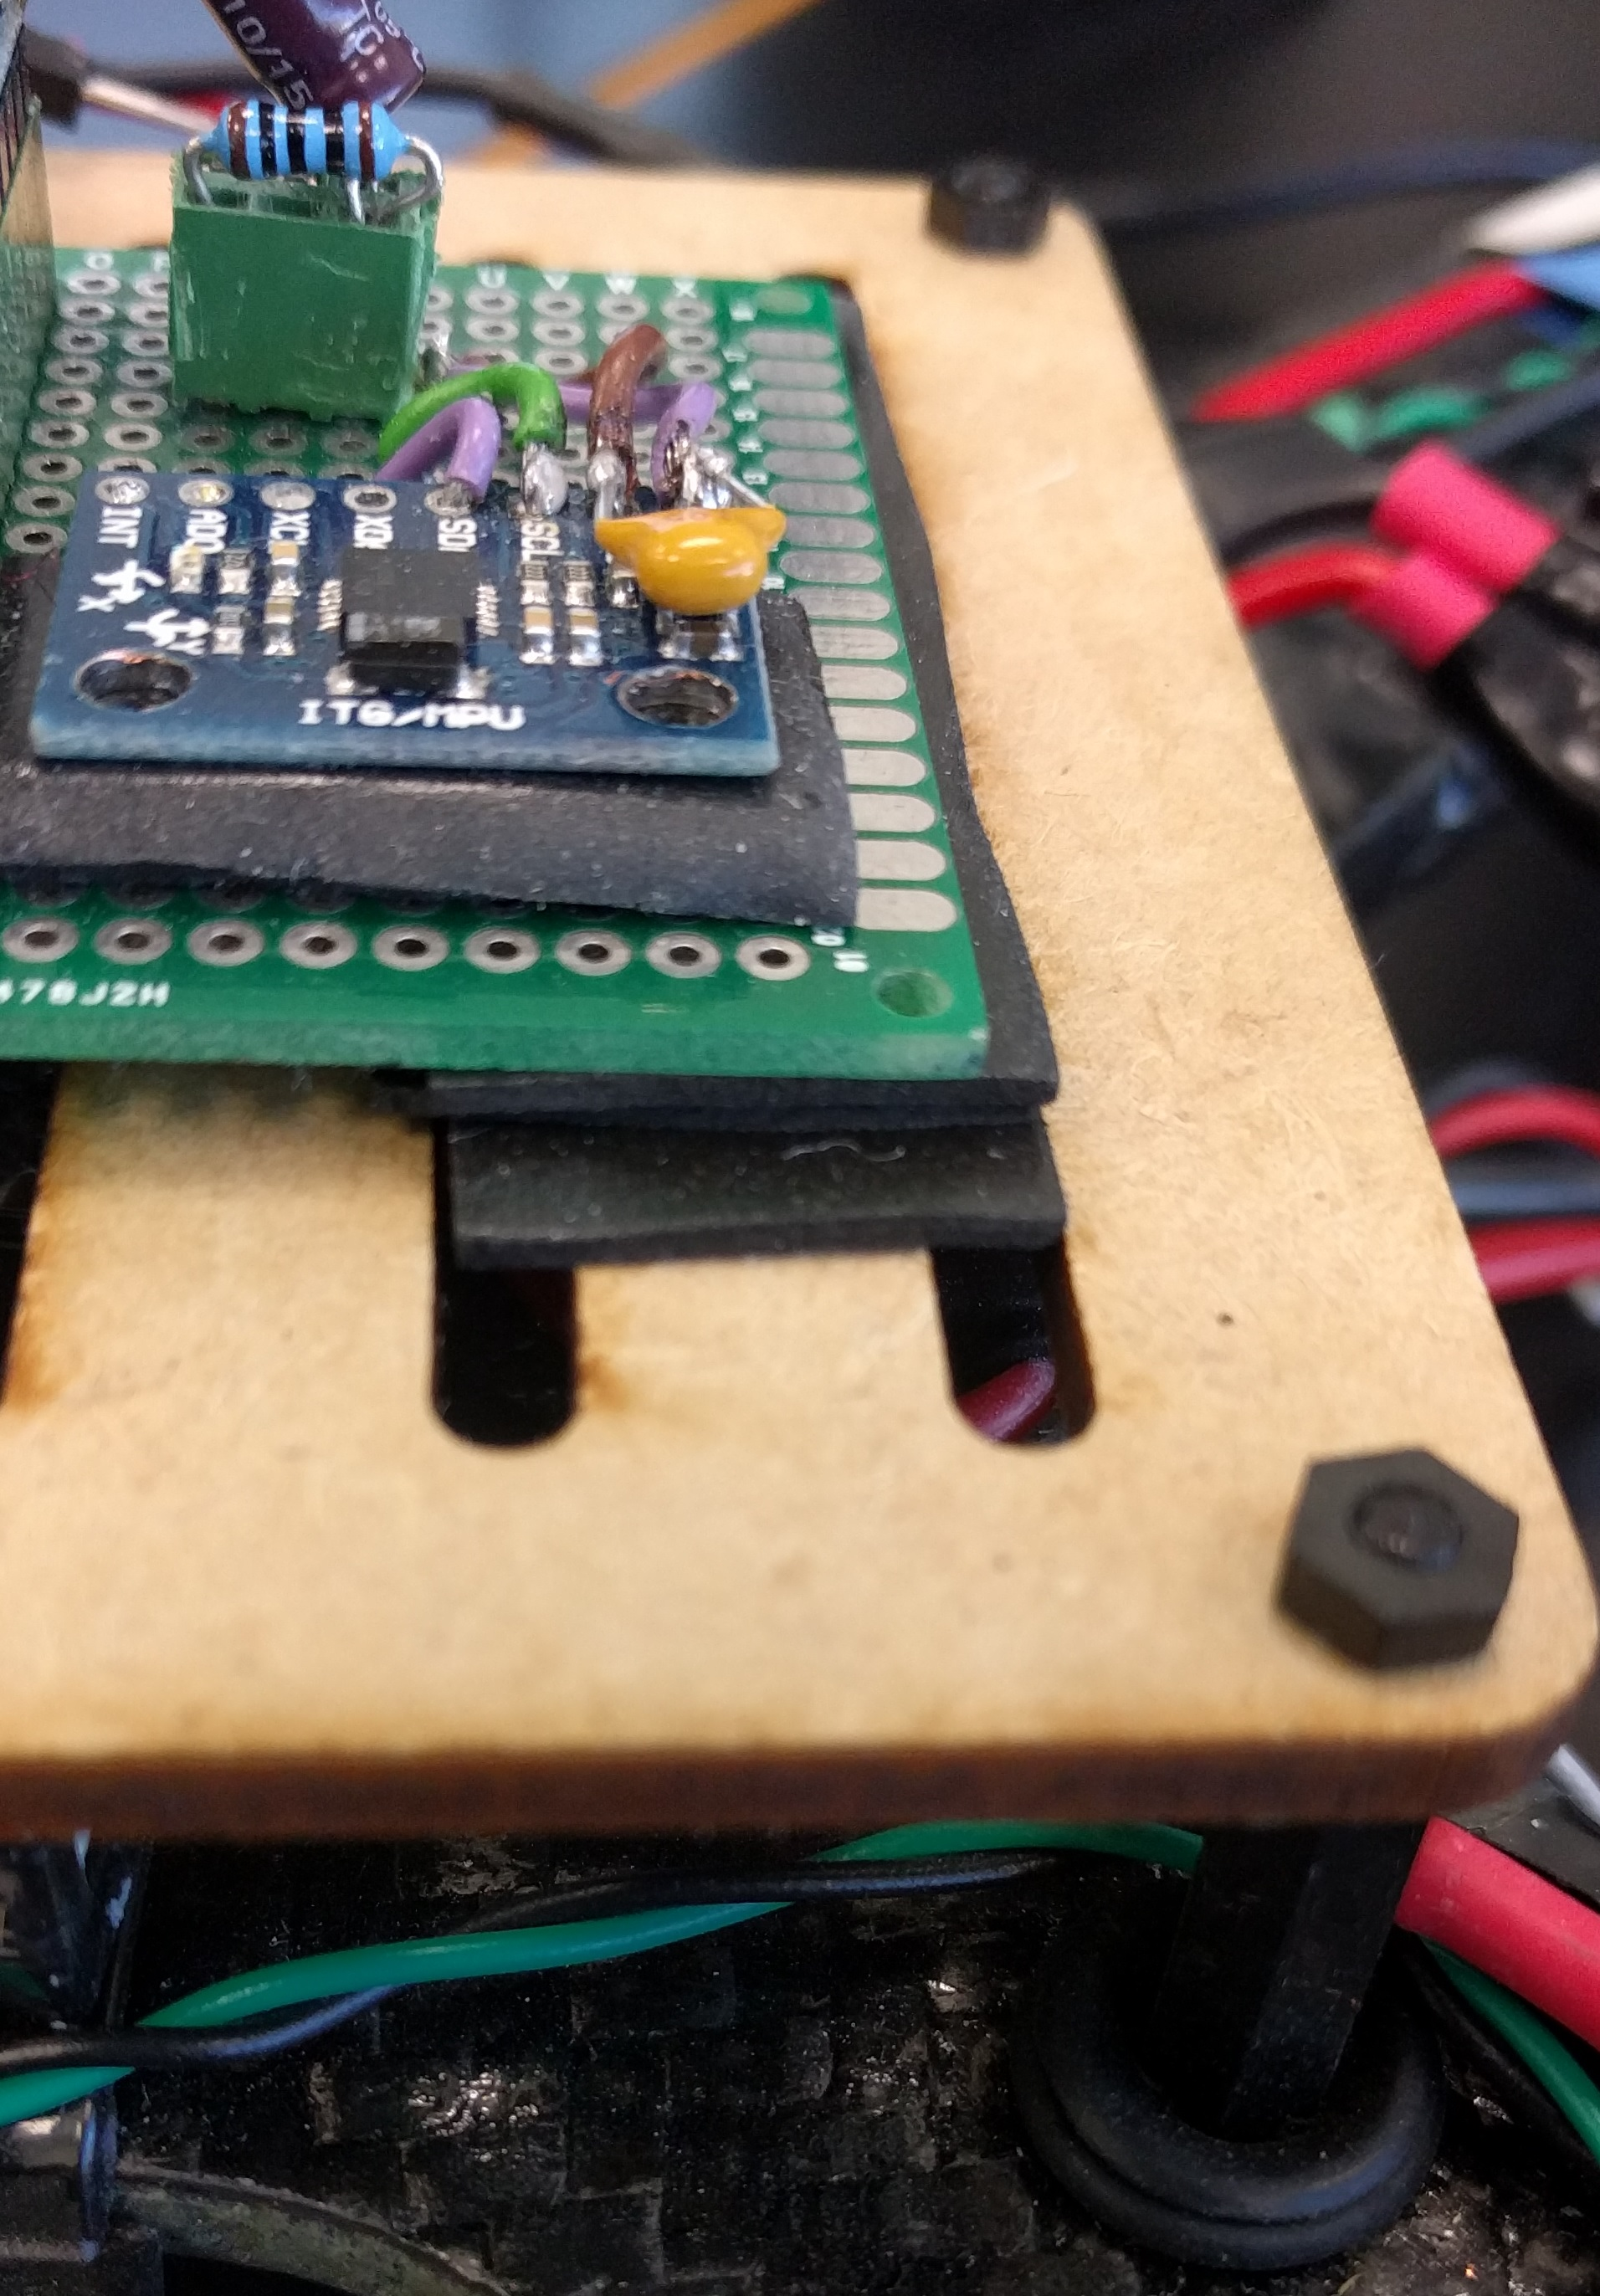
\includegraphics[width = 0.2\textwidth]{NoisePictures/SensorDritt.jpg}
      \caption{IMU mount}
    \label{fig:PIKK2}
\end{figure} 
The physical placement of the IMU is important. The air stream from the propellers can generate vibrations on the sensor, placing it inside a box will reduce air induced vibrations.
\\
\\
The sensor comes with drilled holes which the sensor can be screwed in place,  doing this will make the vibrations worse. The vibrations are carried trough the screw and into the IMU.
\subsection{Electrical Counter Measures}
The stabilization sensors are also exposed to electrical noise and a unstable voltage supply from the $\mu$C. There are several electrical counter measures available to handle this problem.           
\\ \\                   
To minimize the problem with voltage fluctuations an capacitor of 100nF has been added between Vcc and GND on the IMU to smooth out the voltage. An analogue RC low pass filter has also been added to suppress high frequency voltage components. The RC lowpass filter has a cutoff frequency of
\begin{equation}
    F_c = \frac{1}{2\pi RC} = \frac{1}{2\pi 100\Omega (100nF + 4.7\mu F)} = 330 Hz. 
\end{equation}
The filter implementation gave significant more correct and stable readings from the IMU. 
\begin{figure}[H]
    \centering
         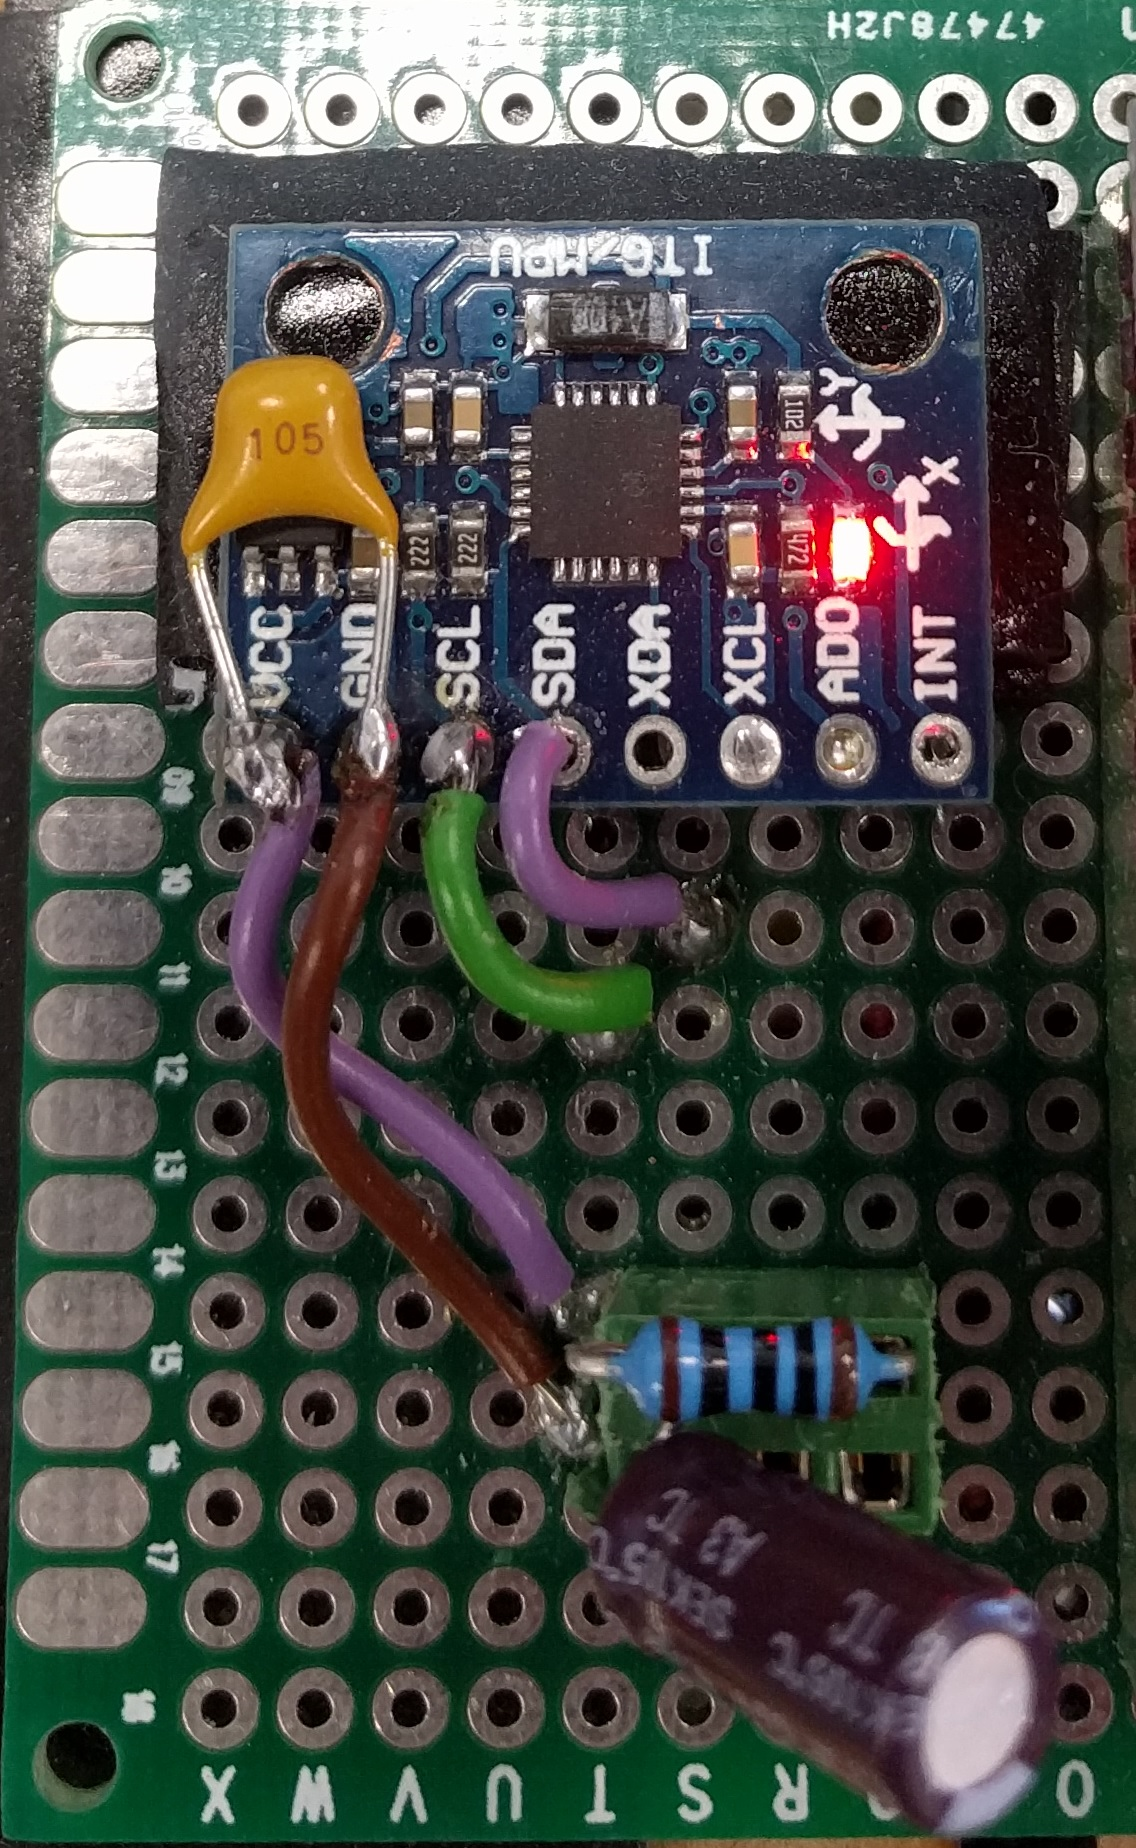
\includegraphics[width = 0.2\textwidth]{NoisePictures/Sensor.jpg}
      \caption{CHANGE THIS PICTURE WITH A KRETSTEGNING}
    \label{fig:PIKK}
\end{figure} 
The quadrotor has several sources that can induce noise on the IMU. The ESC's for example produces noise, which can easily be picked up by the IMU sensor. Therefore it is important to have as short IMU cables as possible in order to limit the electrical noise that can be picked up by the cables. It is also important to place the IMU and cables away from the ESC's because they produce some significant amount noise.
\subsection{Software Counter Measures}

Optimizing a quadrotor mechanically might not be enough to get rid of vibrations. If the quadrotor is optimized mechanically the vibrations must be taken care of in software by means of filtering. There are several filters that are possible to use, the biggest concern when choosing a filter is the time delay and the computational complexity of the filter.
\\
\\
Although several counter measures has been taken on the mechanical and electrical level, the IMU needs processing on the software level. Several methods has been tested out and considered. This includes:
\begin{itemize}
    \item FIR low-pass filter
    \item IIR notch filter
    \item Running average
    \item Complementary filter
    \item Kalman filter
\end{itemize}
Choosing appropriate processing method is always a trade-off between computational complexity, number of samples, and the ability to suppress frequency components and unwanted information. Increasing the number of samples yields a better ability to suppress information, our system is running at 250 Hz which limits the number of samples available for processing. The gyro is being sampled at 8k Hz and the accelerometer is being sampled at 1k Hz. That means that the the maximum number of samples that can be used for processing is 32 and 4 respectively.
\begin{figure}[H]
        \centering
            \begin{minipage}[b]{0.32\textwidth}
                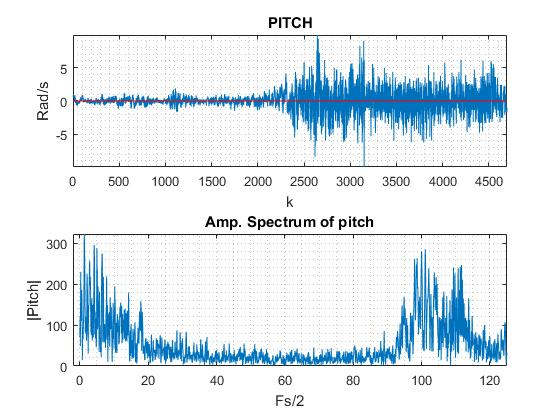
\includegraphics[width = \textwidth, angle= 0]{NoisePictures/PITCH1.jpg}
                \caption{Pitch}
                    %\label{fig:}
            \end{minipage}
            \hfill
            \begin{minipage}[b]{0.32\textwidth}
                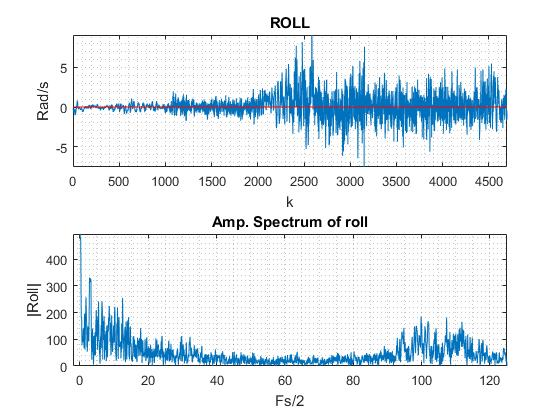
\includegraphics[width =\textwidth, angle =0]{NoisePictures/ROLL1.jpg}
                \caption{Roll}
                %\label{fig:nlknl}
            \end{minipage}
            \hfill
            \begin{minipage}[b]{0.32\textwidth}
                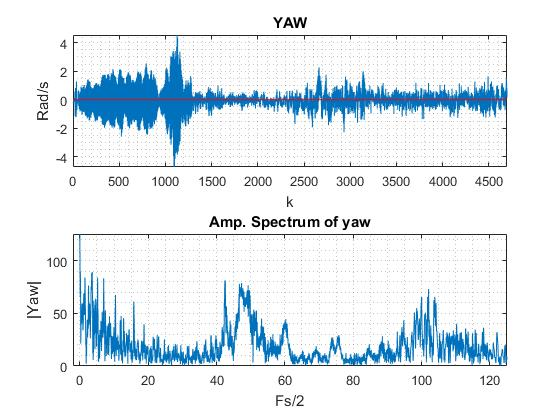
\includegraphics[width =\textwidth, angle =0]{NoisePictures/YAW1.jpg}
                \caption{Yaw}
                %\label{fig:nlknl}
            \end{minipage}
\label{fig:rawData}
\caption{Raw gyroscope data}
\end{figure}
Figure \ref{fig:rawData} shows the raw data from the gyroscope, while the quadrotor is suspended flat on a table, and the thrust is slowly increased to the maximum. The figures shows the data in the time domain on the top and in the frequency domain on the bottom. The time domain plots show that the gyroscope gets inaccurate when the thrust is around 50 \%. Roll and pitch is off by $\pm$ 10 rad/s at the worst. Yaw is of by $\pm$ 6 rad/s at the worst. The data looks symmetric around origo, which implies that averaging the data will effectively reduce the offset. Figure \ref{MovAvg} is the running averaged data sequence of the data in figure \ref{fig:rawData}. This sequence uses 10 samples to compute the mean. This is done step by step of the whole data set.
\begin{figure}[H]
    \centering
         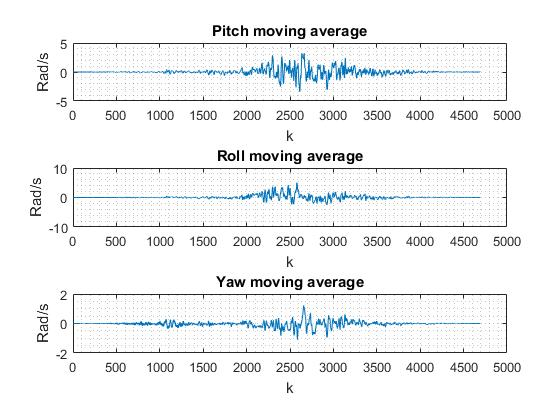
\includegraphics[width = 0.6\textwidth]{NoisePictures/MovingAverageFigure.jpg}
      \caption{Moving average}
    \label{fig:MovAvg}
\end{figure} 
This figure shows that a running average filter will output correct gyro values up to around 50-60\% percent thrust. The mechanical vibrations at this point gets probably to severe, and makes it hard to process in the software level. This limits the agility of the quadrotor and the bottleneck is the mechanical precision of the variable pitch mechanism.
\begin{figure}[H]
        \centering
            \begin{minipage}[b]{0.49\textwidth}
                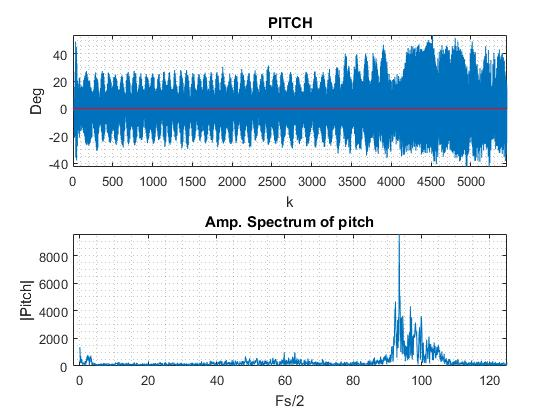
\includegraphics[width = \textwidth, angle= 0]{NoisePictures/PITCHacc.jpg}
                \caption{Pitch}
                    %\label{fig:}
            \end{minipage}
            \hfill
            \begin{minipage}[b]{0.49\textwidth}
                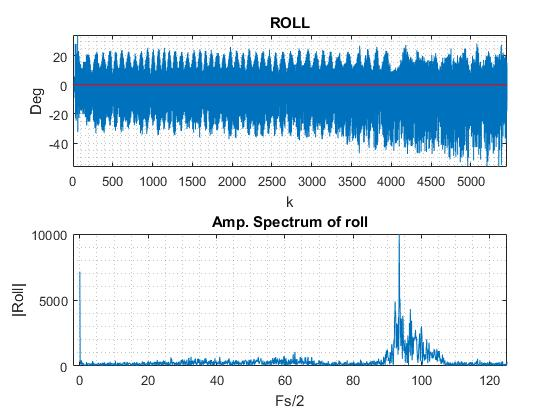
\includegraphics[width =\textwidth, angle =0]{NoisePictures/ROLLacc.jpg}
                \caption{Roll}
                %\label{fig:nlknl}
            \end{minipage}
\label{fig:rawDataAcc}
\caption{Raw accelerometer data}
\end{figure}
Figure \ref{fig:rawDataAcc} shows the raw accelerometer data. This data is also obtained from the quadrotor when it is suspended on a flat table, with the thrust and propeller pitch slowly increasing to the max. The data is clearly wrong and needs some processing in order to be correct. The amplitude spectrum of the data shows that most of the data is in the frequency area of 100 Hz. The information in this frequency area is not of a interest, and is considered as noise. This information must be filtered out. A IIR Notch filter could be useful to filter out this noise. 
\begin{figure}[H]
    \centering
         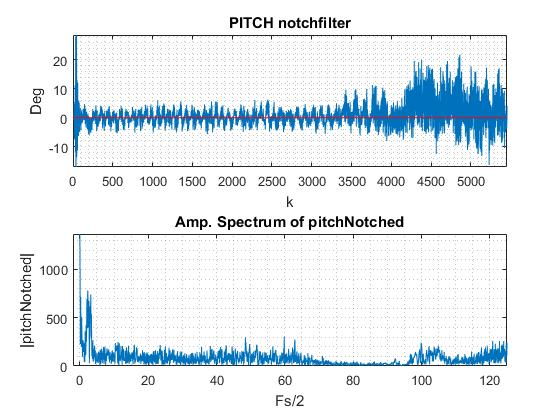
\includegraphics[width = 0.6\textwidth]{NoisePictures/PitchNotchFilt.jpg}
      \caption{Moving average}
    \label{fig:pitchNotchedFig}
\end{figure} 
Figure \ref{fig:pitchNotchedFig} shows the same data sequence as pitch in figure \ref{fig:rawDataAcc} with an IIR notch filter applied to it. The frequency response of the notch filter is seen in figure \ref{fig:notchResp}.

\begin{figure}[H]
    \centering
         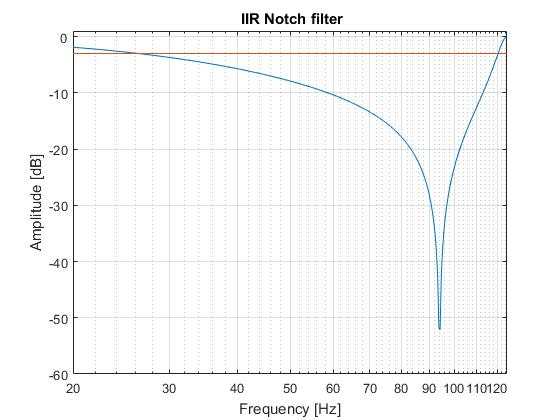
\includegraphics[width = 0.6\textwidth]{NoisePictures/NotchResp.jpg}
      \caption{Moving average}
    \label{fig:notchResp}
\end{figure} 

The data got significant better using this filter  , but there is still a huge offset. The frequency spectrum shows that there is many frequency components spread out in the whole spectrum. Implementing an FIR LP filter will probably yield a better result than using notch filters. Many notch filters is probably required if this approach should work. Implementing a FIR LP filter will yield a much lower total computational complexity.




\begin{comment}
\\
\\
- Solutions (including to the average lowpass filter, the dampening materials attached, and electrical rewiring, we needed more software to overcome this challenge. Complementary filter, rolling average of the three last samples of the last 12 ms did the trick.)

- Filtering
- dampening
- mechanical tuning
- Air slapping
- Need Hæftig presesjon( 10000\^-200000 mm presisjon)
- VIbrations makes autolvling hard because of drift in accelometer
\newline \newline

The following figures show the time and frequency plot of the gyroscope while the throttle is being slowly increased from minimum to maximum value. The plots shows severe vibrations while the throttle is ~$\ge$ 50$\%$.


By investigating figure \ref{yaw1} it can be seen that much of the noise can be filtered out by means of a running average filter or a median filter. Yaw seems to have most of the noise, this is probably due to a throw in the shaft that pushed the variable pitch mechanism. Figure \ref{fig:Average1} shows the signals averaged. 
\newline \newline
The sample rate of the IMU is limited to 250 Hz. That makes is challenging to filter the IMU data in software. An anti-aliasing filter is required because there will be frequency components over $\frac{Fs}{2}$.
\begin{figure}[H]
    \centering
         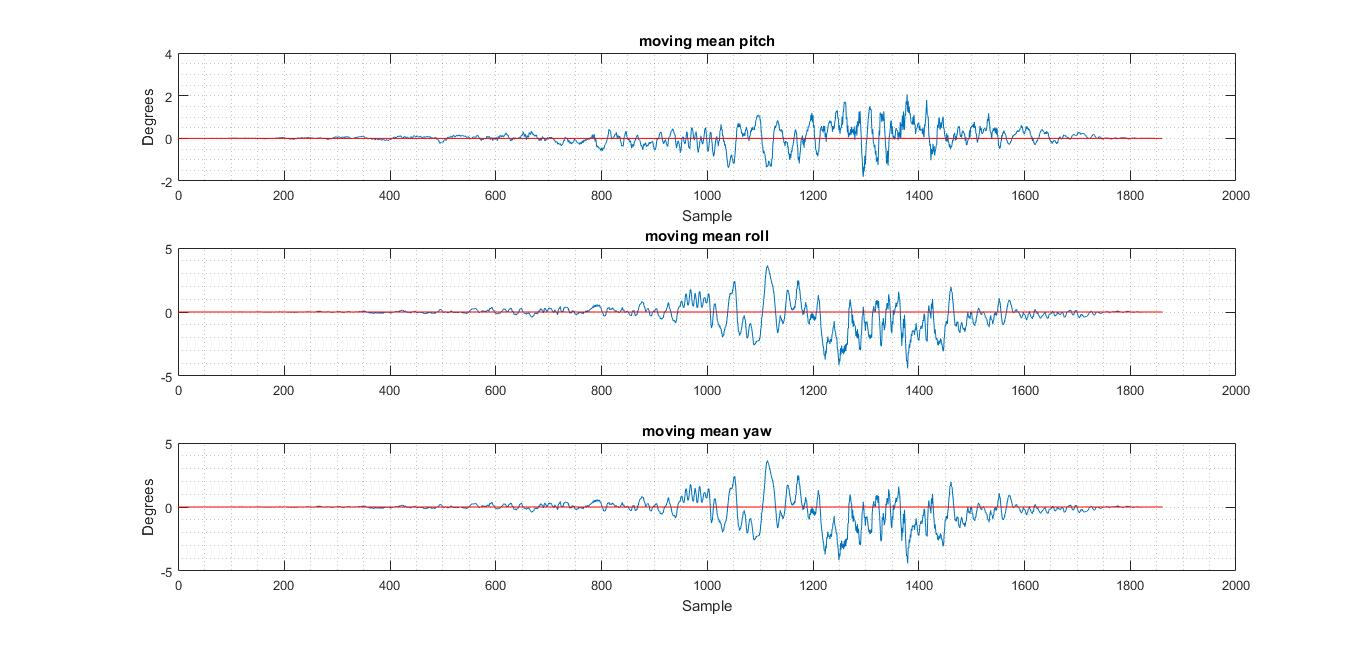
\includegraphics[width = 0.9\textwidth]{NoisePictures/Average1.jpg}
      \caption{Kis}
    \label{fig:Average1}
\end{figure}

\end{comment}

\subsection{Conclusion}

Vi er eid...............................


\subsection{Solution For FPQ}
For the fixed pitch quadrotor the solution to the vibration challenges was a combination of different filters and methods to reduce the noise. The filters considered were; Kalman, complementary, IIR notch filters, average, median and FIR LP. The aim has been to reduce the magnitude of incorrect values caused by the disturbances on the sensor from motor vibrations. \\
\\
Several IMU sensors have been considered and tested for this project.The sensor chosen for the project had errors and would occasionally freeze and give incorrect data. This made it more difficult to select the right filter and more difficult to understand the impact it would have. 


*insert vibration graph without props*
\\
The raw data from the sensor was analyzed by taking different RPM levels and registering the noise in each level. This information was analyzed and showed that the entire resonance frequency range was covered, excluding the IIR notch filter from evaluation.  To overcome the vibrations from the rotating propellers a lowpass filter and exponentially weighted moving average filter was simulated in matlab. The simulated results gave good data, and the filters was shortly after implemented in the flight controller. These filters where then tested, and gave a $\pm$ 4 degrees in the worst case scenario. This is not good enough from what we initially wanted, which is less than $\pm$ 1 degrees of error. \\
\\
The real world is unfortunately not as pure as what simulations can show. It is more noisy and ugly. We started implementing an average filter to achieve results closer to the actual values. We simulated different sample sizes. The average filter was implemented in the flight controller as a generic function with the possibility to change sample size and the amount of spikes to be removed. The spikes was another attempt at removing the noise, we experienced some values as very high compared to the rest. Because of these spikes, we added functionality to remove some of largest and lowest number of spikes. This implementation was tested and we ended up with an average of 20 samples and removing 3 spikes. The sampling speed of the gryo is 1kHz. Measuring 20 samples and taking the average gave us an update frequency of 50Hz. This compromise lowers the overall agility of the quadrotor but gives us more reliable data. Removing the spikes costs a lot of computational power. This is because all of the samples must be sorted, and gave little back compared to the other methods discussed. This was in the final implementation excluded from the code.\\
\\
Other filters discussed but not implemented and tested is Kalman and IIR notch filter. Kalman is considered as one of the best filters for quadrotors by many. (source?) Kalman filter takes extra computational time, especially extended Kalman filter, but gives in return very accurate data. The expected time to get a good Kalman filter inplace was also considered to take more time than other filters. For this reason it was not implemented and tested. IIR notch is an other filter considered but not used. The reason for this is because we don't have any specific resonance frequencies to filter out. \\
